\documentclass[11pt]{article}

\marginparwidth 0.5in
\oddsidemargin 0.25in
\evensidemargin 0.25in
\marginparsep 0.25in
\topmargin 0.25in
\textwidth 6in
\textheight 8in

\usepackage{amsmath, amssymb}
\usepackage{upgreek}
\usepackage{latexsym}
\usepackage{graphicx}

\begin{document}
\begin{flushleft}
Juan Miguel C. Manalo \\
2014-40093 \\
CS 145 THWMXY-HONOR
\end{flushleft}

\begin{center}
\textbf{CS145 Lab Exercise 3: Wireshark Lab - Internet Protocol and Traceroute Operation}
\end{center}

\begin{enumerate}
\item
9 routers, not including the server hosting the Philippine Daily Inquirer.
\begin{center}
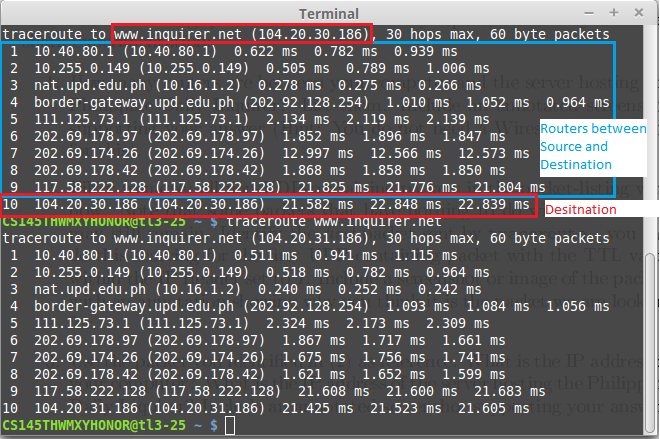
\includegraphics[scale=0.5]{Q1}
\end{center}

\item
Packet \#7
\begin{center}
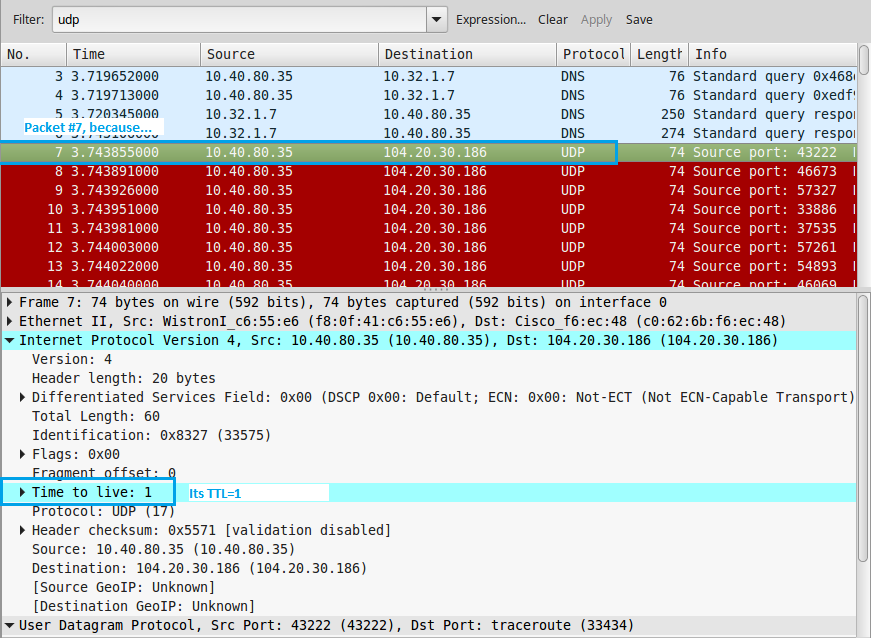
\includegraphics[scale=0.4]{Q2}
\end{center}

\item
IP Address (Computer): \textbf{10.40.80.35} \\
IP Address (Website): \textbf{104.20.30.186}
\begin{center}
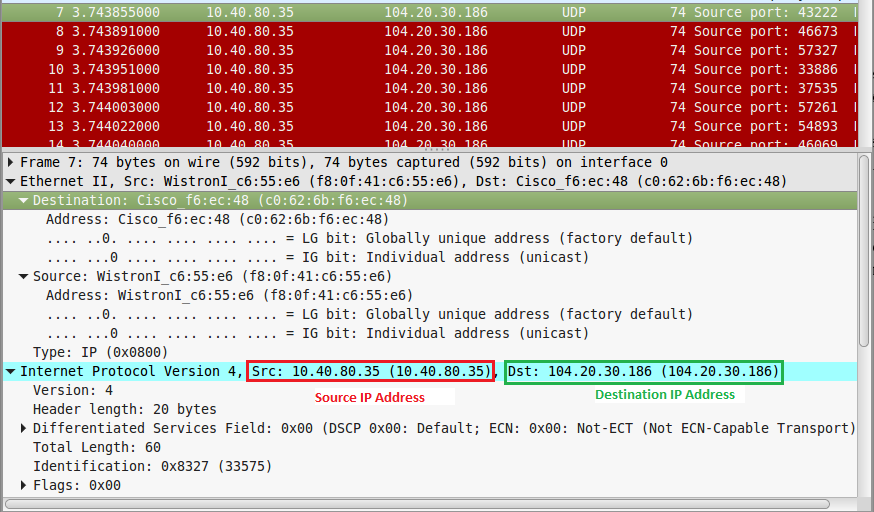
\includegraphics[scale=0.4]{Q3}
\end{center}

\item
IP Header: \textbf{20 bytes} \\
IP Datagram Payload: \textbf{40 bytes} \\
As annotated, the total length of the IP Datagram is 60 bytes. To get the payload, subtract the IP Header bytes from the total length of the datagram. Hence, $60 - 20 = 40$ bytes.
\begin{center}
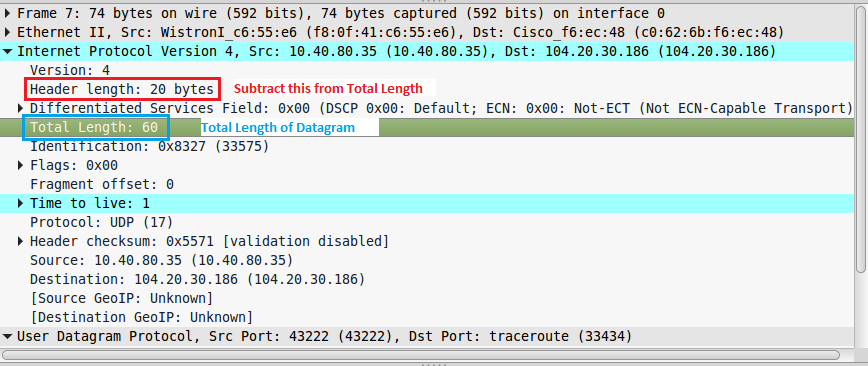
\includegraphics[scale=0.4]{Q4}
\end{center}

\item
The Identification and the Checksum. They are as follows:
\begin{itemize}
\item{Packet \#7: 0x8327 (Identification), 0x5571 (Checksum)}
\item{Packet \#8: 0x8328 (Identification), 0x5570 (Checksum)}
\item{Packet \#9: 0x8329 (Identification), 0x556f (Checksum)}
\end{itemize}

\item
The Internet Protocol Version, Header Length, Differentiated Services Field, Flags, TTL, Protocol, Source, and Destination.

\item
The values in the Identification field increase by 1 each succeeding packet.

\end{enumerate}

\end{document}